\documentclass[letterpaper, 11pt]{article}

% set version variable
\newcommand{\versionnumber}{0.1}

% russian language
\usepackage[utf8]{inputenc}
\usepackage[T2A]{fontenc}
\usepackage[english, russian]{babel}
\usepackage{algorithmicx}
\usepackage{algpseudocode}
\usepackage{graphicx}
\usepackage{caption}
\usepackage{subcaption}
\usepackage{amsmath}


% math
\usepackage{amsmath}

\usepackage{amssymb} % some math symbols


% enumerate
\usepackage{enumerate}

% set type and margins of the page
\usepackage{geometry}  % document margins
\geometry{letterpaper, left=1.4in, right = 1.4in, top = 1.7in, bottom = 1.7in}

% color links in content
\usepackage{hyperref}
\hypersetup{
    colorlinks=true,
    linkcolor=red,
    urlcolor=blue,
    linktoc=all
}

% indent at first \par after section
\usepackage{indentfirst}

% fixed table and figures in section
\usepackage{float}

% colors
\usepackage{color}
\usepackage[usenames,dvipsnames]{xcolor}

\newcommand{\prob}{\mathrm{P}}
\newcommand{\expe}{\mathrm{E}}
\newcommand{\var}{\mathrm{D}}
\newcommand{\tr}{\mathrm{tr}}
\newcommand{\KK}{\mathbf{K}}
\newcommand{\XX}{\mathbf{X}}
\newcommand{\MM}{\mathbf{M}}
\newcommand{\Cov}{\mathrm{Cov}}
\newcommand{\Var}{\mathrm{Var}}

% paragraph indent
\setlength{\parskip}{0.5em}

\title{\large{Краткий конспект}\\
\LARGE{LAFF}}
\date{6 апреля, 2016}
\author{\underline{Д. Ищенко\thanks{МФТИ}} \and Б. Коварский\footnotemark[1]
\and И. Алтухов\footnotemark[1] \and Д. Алексеев\footnotemark[1]}

\begin{document}
\maketitle
\thispagestyle{empty}
\clearpage

% let's go
\section{Задача}

\textbf{Given}: Two protein strings $s$ and $t$ in FASTA format (each having length at most 10,000 aa).

\textbf{Return}: The maximum local alignment score of $s$ and $t$, followed by substrings $r$ and $u$ of $s$ and $t$, respectively, that correspond to the optimal local alignment of $s$ and $t$

\textbf{Use}:
\begin{enumerate}
\item
The BLOSUM62 scoring matrix.
\item
Gap opening penalty equal to 11.
\item
Gap extension penalty equal to 1.
\end{enumerate}

If multiple solutions exist, then you may output any one.

\section{Оптимизация памяти}
Начнем издалека, рассмотрим глобальное выравнивание, для которого нужно вычислить только значение скоринга. Нужно ли нам хранить всю матрицу $n \times m$, что, очевидно, является $O(nm)$? Допустим, мы заполняем ее проходом по строкам. Для каждой ячейки мы проверяем три перехода: через гэп из <<левой>>, через гэп из <<верхней>> или по диагонали из <<левой-верхней>> ячейки. Т.е. для вычисления скоринга нам достаточно хранить значения скоринга в текущей и предыдущей строках. При переходе к новой строке, обновить (переприсвоить) предыдущую и т.д. Финальным глобальным скорингом будет значение в последней клетке. Итого всего необходимо хранить $2m$ элементов, т.е. $O(m)$.

Выглядеть это будет примерно так:
\begin{verbatim}
  prev_row = [...] # не забыть правильно задать первую (нулевую) строку
  for i in 1..nrow
    cur_row = [...] # правильно задать первый (нулевой) элемент
    for j in 1..ncol
      cur_row[j] = max(...)
    prev_row = cur_row
  
  S = prev_row[m-1]
\end{verbatim}

Что будет, если выравнивание не глобальное, а локальное? И нам опять нужно только значение скоринга. Необходимо найти абсолютный максимум во всей матрице, но т.к. всей матрицы у нас нет, будем проверять является ли значение в текущей ячейке максимальным на каждом шаге.

\begin{verbatim}
  S = 0
  prev_row = [...] # не забыть правильно задать первую строку
  for i in 1..nrow
    cur_row = [...] # правильно задать первый (нулевой) элемент
    for j in 1..ncol
      cur_row[j] = max(...)
      if cur_row[j] > S:
        S = cur_row[j]
    prev_row = cur_row
\end{verbatim}

Отлично, а что если нас интересует не только скоринг, но и подстроки из выравниваемых $s$ и $t$, которые дают этот скоринг? Обратим внимание, что нас интересует не само выравнивание, а \textit{только подстроки}, т.е. нам не нужно расставлять гэпы, а значит достаточно знать только начальные и конечные координаты подстрок из $s$ и $t$. Для удобства будем пользоваться одним индексом для кодирования положения ячейки в матрице, т.е. не будем указывать отдельно строку и столбец, а будем работать с $icell = irow \cdot ncol + icol$, где $irow$ -- индекс строки, $icol$ -- индекс столбца, $ncol$ -- кол-во столбцов в матрице. Это равносильно тому, что мы пронумеровали ячейки матрицы следующим образом:

\begin{verbatim}
 0   1   2   3   4   5
 6   7   8   9  10  11
12  13  14  15  16  17
\end{verbatim}

Получить номер строки и столбца из $icell$ тоже легко, $irow = icell \; / \; ncol$, $icol = icell \; \% \; ncol$, где $/$ -- целочисленное деление, $\%$ -- остаток от деления.

Итак, нам нужно для каждой ячейки узнать откуда <<начинался>> наш путь в нее (т.к. выравнивание локальное, то это не обязательно ячейка $[0, 0]$). Для этого создадим еще одну матрицу $T : n \times m$, в которой будем хранить <<координату начала>> -- ячейку матрицы (будем использовать вышеописанную обощенную координату), из которой начинался путь. И, опять же, нам не нужно хранить всю матрицу, а, по аналогии с матрицей скорингов, только текущую и предыдущую строки этой матрицы. Если мы пришли в текущую $[i][j]$ клетку слева, то координата начала для текущей равна координате начала левой $T[i][j] = T[i][j - 1]$, если сверху -- то верхней $T[i][j] = T[i - 1][j]$, если по диагонали: $T[i][j] = T[i - 1][j - 1]$, новое значение появляется только в случае, если мы пришли сразу из нуля (т.е. максимальный скоринг равен $0$), тогда $T[i][j] = i \cdot ncol + j$.

Код немного усложнится, нам понадобится два дополнительных массива $prev\_st\_row$ и $cur\_st\_row$ (для предыдущей и текущей строки матрицы $T$), а также при поиске максимального значения, мы должны запоминать не только само значение, а еще и старт для него, а также саму координату максимума. Код будет выглядеть примерно так:

\begin{verbatim}
  S = 0
  prev_row = [...] # не забыть правильно задать первую строку
  prev_st_row = [...] # подумать, как задать первую
  for i in 1..nrow
    cur_row = [...] # правильно задать первый (нулевой) элемент
    cur_st_row = [...] # правильно задать первый (нулевой) элемент
    for j in 1..ncol
      cur_row[j] = max(...)
      cur_st_row[j] = ... # задать в соответствии тому, откуда пришли
      
      if cur_row[j] > S:
        S = cur_row[j]
        start = cur_st_row[j]
        end = i * ncol + j
    prev_row = cur_row
    prev_st_row = cur_st_row
\end{verbatim}

Зная $start$ и $end$, нам ничего не стоит вычислить соответствующие им номера столбцов и строк, а это и будут индексы начала и конца подстрок (не перепутайте, кто за что отвечает и нужно ли добавлять или отнимать единицы от индексов).

\section{Аффинные гэпы}

Теперь, когда мы разобрались, как оптимизировать необходимую оперативную память, перейдем к аффинным гэпам. В чем основная сложность? В том, что мы можем перейти в ячейку не только из ее <<трех соседей>> и нулевой клетки, а еще и из любой <<левой>> клетки в ее строке и любой <<верхней>> клетки в ее столбце. Такая проверка приведет нас к $O(n^3)$ (Рис. 1), что на предложенных строках не представляется возможным выполнить за отведенное время.

\begin{figure}[H]
  \center{
  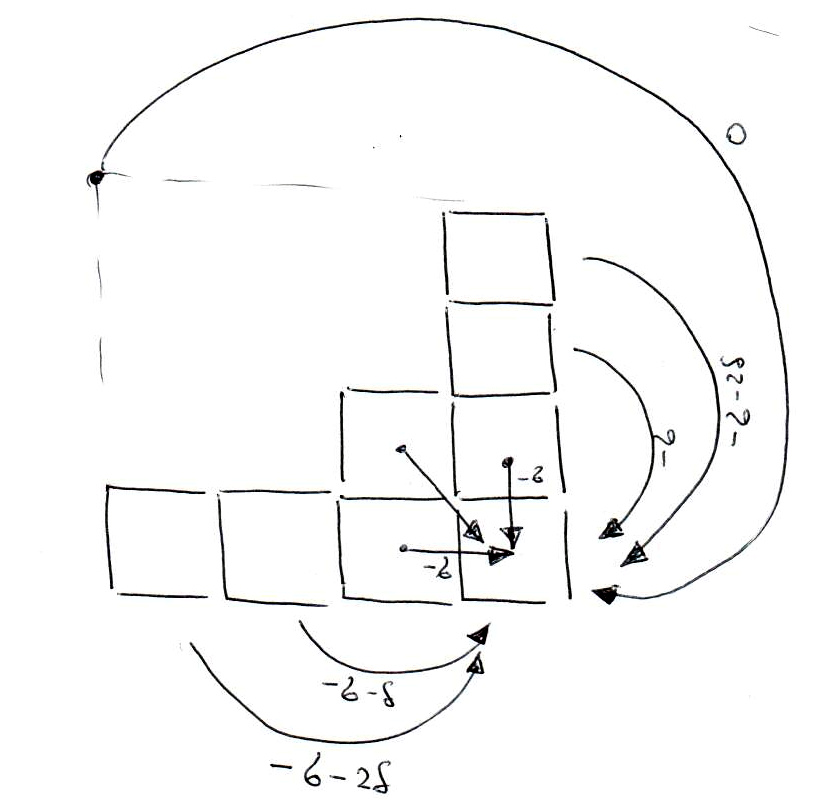
\includegraphics[scale = 0.85]{fig/laff1.jpg}
  }
  \caption{Подход с проверкой всех возможных переходов $O(n^3)$. Штраф за открытие гэпа $\sigma$, за продление $\delta$.}
\end{figure}

Ограничимся рассмотрением переходов только по строке. Допустим, мы сравниваем между собой <<длинный>> переход в ячейку с координатой $z$ из двух различных ячеек с координатами $x$ и $y$ и соответсвтующими в них значениями скоринга $S_x$ и $S_y$ (Рис. 2).

\begin{figure}[H]
  \center{
  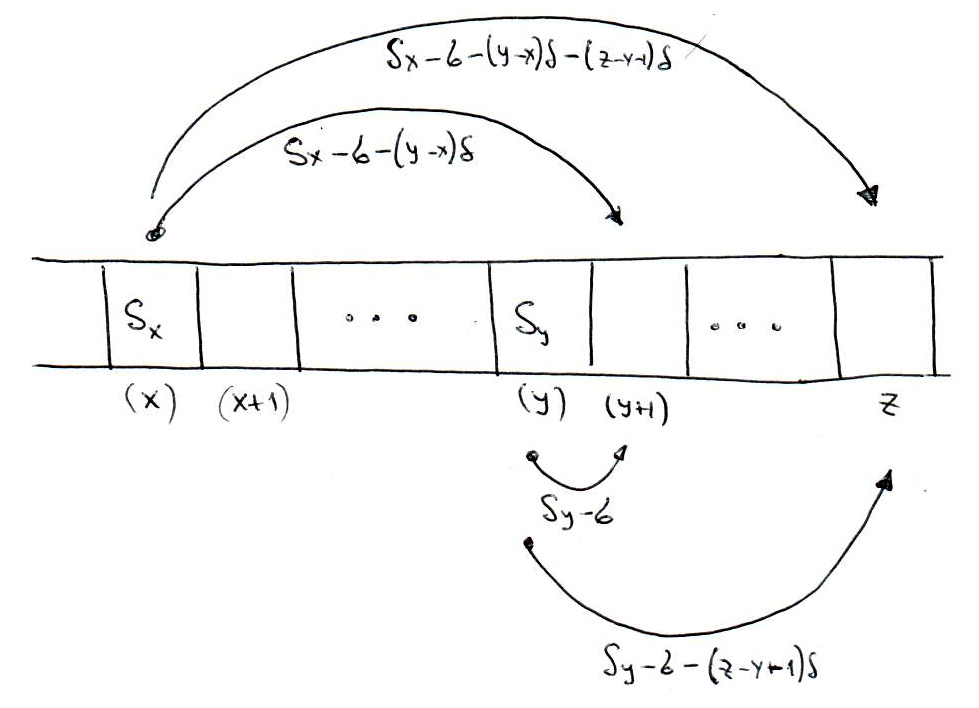
\includegraphics[scale = 0.85]{fig/laff2.jpg}
  }
  \caption{Переход в $z$ из ячеек с координатами $x$ и $y$ и скорингами $S_x$ и $S_y$.}
\end{figure}

На что тут стоит обратить внимание: чтобы прийти из $x$ или $y$ в $z$ нужно сначала из них дойти в $(y+1)$ ячейку, а из нее уже <<продлиться>> в $z$ со штрафом $(z - y - 1)\delta$. А значит, если уже в $(y + 1)$ ячейке скоринг из $x$ будет выше, то и в $z$ мы придем с большим скором из $x$ (и наоборот). И такая аналогия для всех остальных клеток с координатой меньше, чем $y$ (всегда нужно дойти до $(y+1)$ и потом <<продлиться>>). Представим, что $(y + 1) = (z - 1)$, т.е. рассмотрим соседнюю слева клетку от $z$. Отсюда следует, что проверяя переход в $z$ мы должны для строки \textit{помнить лишь только одну <<лучшую>> ячейку} до $z$ из которой имеет смысл проверять переход. А лучшая для $z$ в строке, это лучшая из двух: (i) лучшая для $(z - 1)$ ячейки с дополнительным единичным продлением или (ii) открытие нового гэпа из $(z-1)$ ячейки. Приходим к рекурсии.

\begin{figure}[H]
  \center{
  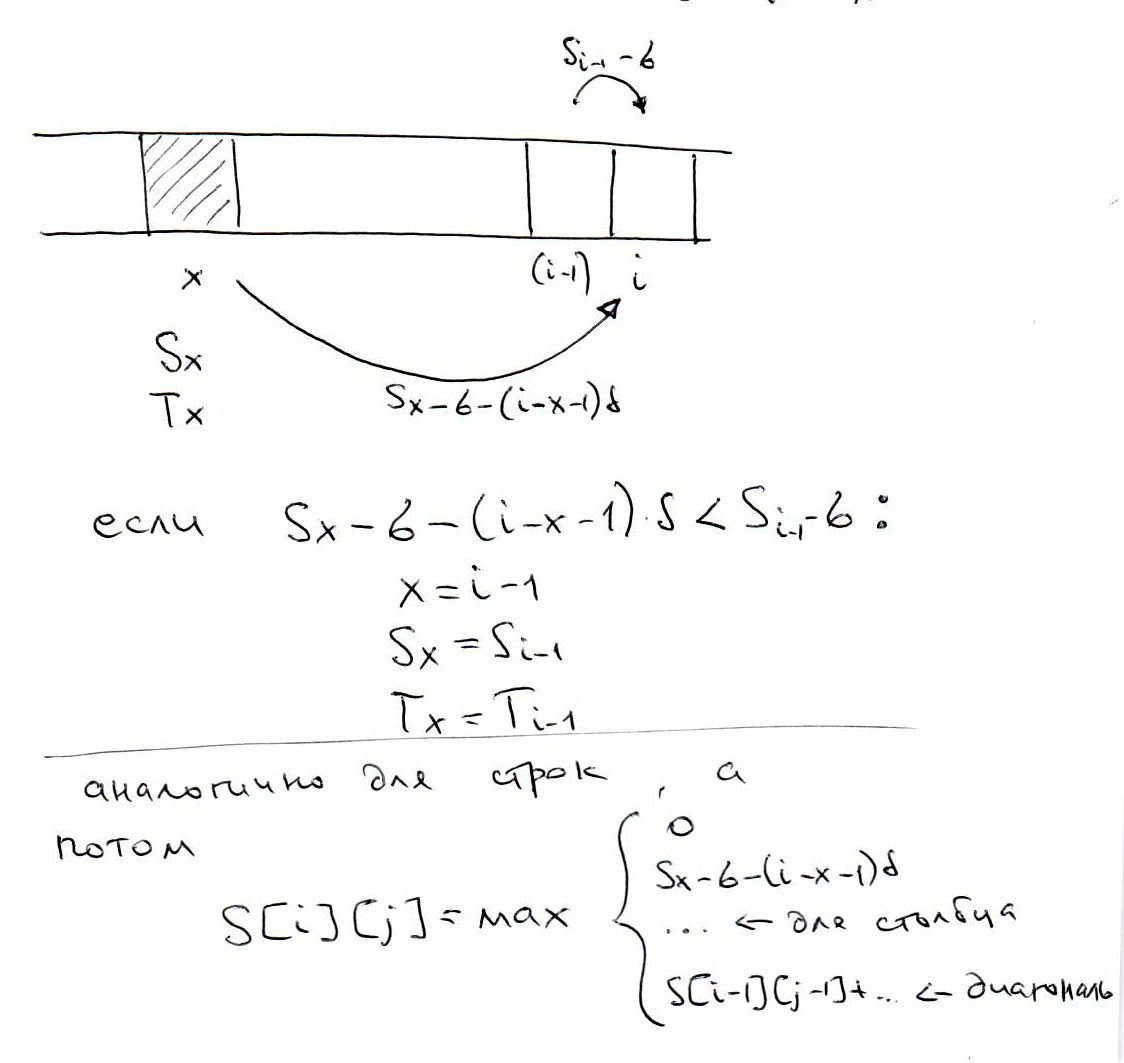
\includegraphics[scale = 0.85]{fig/laff3.jpg}
  }
  \caption{Проверка на <<лучшую>> для открытия гэпа ячейку в строке для $i$-ой ячейки.}
\end{figure}

Для лучшей ячейки в строке мы должны хранить три числа: ее координату ($x$), скоринг в этой ячейке ($S_x$) и значение <<старта лучшего пути>> ($T_x$) (помним, что нам нужно выводить подстроки, а значит нужно знать стартовую ячейку). Прежде чем присвоить $S[i][j]$, проверим, выгодней нам продлить путь из предыдущей <<лучшей>> или открыть новый гэп из соседней. Если открыть новый выгоднее, то <<лучшая>> ячейка теперь соседняя (переприсваиваем $x$, $S_x$ и $T_x$). Аналогичную операцию нужно сделать для столбца, единственное отличие, что т.к. мы идем по строкам, то нам необходимо помнить все тройки ($x, S_x, T_x$) для каждого столбца, т.е. будет три массива длиной $m$, $x[1..m]$, $S_x[1..m]$ и $T_x[1..m]$ и находясь в $j$-ом столбце мы будем работать с тройкой $x[j]$, $S_x[j]$ и $T_x[j]$, а логика точно такая же. После проверок на <<лучшие>> клетки, мы делаем проверку на сам скоринг в клетке $S[i][j]$, но уже не забоитмся о длинных и коротких гэпах, а просто находим максимум из четырех значений: (i) нулевой, (ii) по диагонали, (iii) из лучшей слева и (iv) из лучшей сверху (они у нас уже переприсвоены). В зависимости от перехода переприсваиваем и старт $T[i][j]$ и проверяем, как и ранее, не является ли текущий скоринг абсолютным максимумом.

В конце мы получаем максимальный скоринг и координаты $start$ и $end$ и выводим подстроки.

Победа!

\textit{P.S. Будьте внимательны при инициализации массивов $x[1..m]$, $S_x[1..m]$ и $T_x[1..m]$ и задании начальных значений для $x, S_x, T_x$ при движении по строке. И, в целом, будьте внимательны :)}


\end{document} 
